\documentclass[12pt]{article}

%packages
%package for drawing diagrams manually
\usepackage{tikz}
\usepackage[margin = 1in]{geometry}
%package for all the math symbols and font styles
\usepackage{amsfonts,amsmath,amssymb}
%package for preventing latex to use hyphenated words
\usepackage[none]{hyphenat}
\usepackage{listings}
\usepackage{color} %red, green, blue, yellow, cyan, magenta, black, white
\definecolor{mygreen}{RGB}{28,172,0} % color values Red, Green, Blue
\definecolor{mylilas}{RGB}{170,55,241}

% Package for writing multiple authors along with their affiliations
\usepackage{authblk}

%\usepackage{footmisc}

% Report Parameters
% Report Title
\def\reporttitle{\textbf{Impact Location Prediction using Deep Learning with the aid of Convolutional Neural Network (CNN)}}

%Header and footer
\usepackage{fancyhdr}

%package for graphics (pictures)
\usepackage{graphicx}

\usepackage{float}

\parindent 0ex %command for removing any indentation in all the paras

\pagestyle{fancy}
\fancyhead{}
\fancyfoot{}
\fancyhead[L]{\textsc{\reporttitle}}
%\fancyhead[R]{\textit{Ashutosh Mukherjee}}
\fancyfoot[C]{\thepage}


\usepackage[utf8]{inputenc}
\usepackage[T1]{fontenc}

% \usepackage{titling}
% \predate{}
% \postdate{}

% Keywords command
\providecommand{\keywords}[1]
{
  \small	
  \textbf{\textit{Keywords---}} #1
}

% Package for referencing
\usepackage{biblatex}

\usepackage{makecell}

\usepackage[font=small, labelfont=bf]{caption}
\usepackage{subcaption}


\begin{document}
\title{\reporttitle}
\author[1]{\textbf{Ashutosh Mukherjee}}
\author[2]{\textbf{Neel Savla}}
\author[2]{\textbf{Raj Khamkar}}
\author[2]{\textbf{Vibhav Singhal}}
\affil[1]{\small{\textit{Computer Aided Conception and Production in Mechanical Engineering, RWTH Aachen University, Aachen, Germany}}}
\affil[2]{\small{\textit{Management and Engineering in Computer Aided Mechanical Engineering, RWTH Aachen University, Aachen, Germany}}}
\date{\vspace{-5ex}} % Removes the date and covers up the empty space using vspace
\maketitle

\begin{abstract}
\noindent
It has become more important than ever to build highly sustainable systems and structures. One technique to warrant the safety and durability of any structure without over-engineering the components, is to have a continuous health monitoring system that can sense any alarming peripheral impact which could lead to significant damage at later stages of the structure's life. This study aims to predict impact location from piezoelectric sensor data placed symmetrically on the study specimen using Artificial Neural Network (ANN). This can then be implemented in operation in order to, monitor the structural health of static as well as dynamic structures. 
\end{abstract} \hspace{10 pt}

\keywords{deep learning, convolutional neural network, structural health monitoring system, architecture comparison, balanced data}

\section{Introduction}

\setlength{\parindent}{20pt}
To facilitate sustainability on all fronts, the next generation of machines and structures must be more robust and long-lasting. This can be achieved by a continuous health monitoring system. The prediction of an impact location on a static or a dynamic system by a foreign object constitutes the basic purpose of a structural health monitoring system\cite{1}\cite{2}. The solution to the problem entails obtaining vibrational sensor data that is fed to a computationally intelligent system capable of predicting the site of the impact relative to the system thus, keeping a log of the stresses developed in the structure over the period of its operation due to such impacts. In this research project, we aim to create, compare and identify an optimum computationally intelligent system between Convolutional Neural Network (CNN)\cite{3}, Recurrent Neural Network (RNN)\cite{4} and Feed Forward Neural Network (FFNN)\cite{5} to predict the location of the site of impact on the structure under observation.

\par 
\noindent
For the purpose of this research project, vibration patterns generated by a controlled impact caused by a steel ball of known size and dropped from a specific height on an aluminium plate were recorded using four symmetrically placed piezoelectric transducers (Fig.~\ref{expSetup}). The entire experiment was also simulated to generate numerical data which along with the experimental data was then fed to the aforementioned Artificial Neural Networks (ANN) for the prediction of impact site using computational intelligence.  
\\
\begin{figure}[h!]
\begin{center}
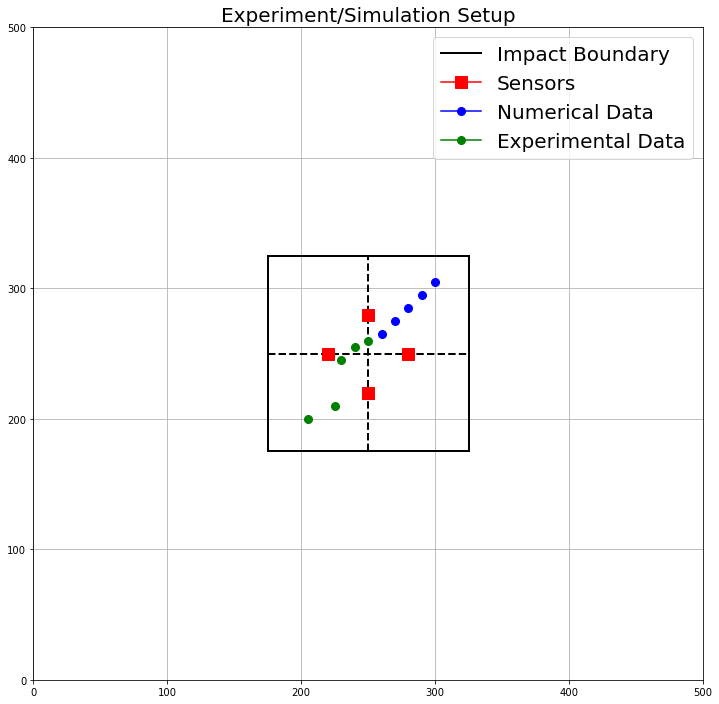
\includegraphics[scale=0.4]{"Images/Experimental setup.png"}
\caption{A model of the experiment set-up used for the numerical as well as the experimental data acquisition}
\label{expSetup}
\end{center}
\end{figure}   

\section{Methods}

For this study, regression models\cite{6} were built to predict the X and Y coordinates of the impact locations with respect to the mutually set origin of the experimental setup consisting four piezoelectric transducers using FFNN, RNN and CNN. Models were compared on prediction accuracy and variation of each model by training them on numerically simulated and experimental data. All the three architectures were tested on a prediction dataset where the impact coordinates were initially unknown and were made available later for validation purposes. The best suited neural network model was then further extended to check the prediction accuracy of the X and Y position of impact using independent neural networks as compared to a single neural network model. Further optimisation of the selected model was then performed by balancing the data in each quadrant for training the neural network. This workflow is depicted in the flowchart below (Fig.~\ref{flowchart}).
\par
\pagebreak

\begin{figure}[h!]
\begin{center}
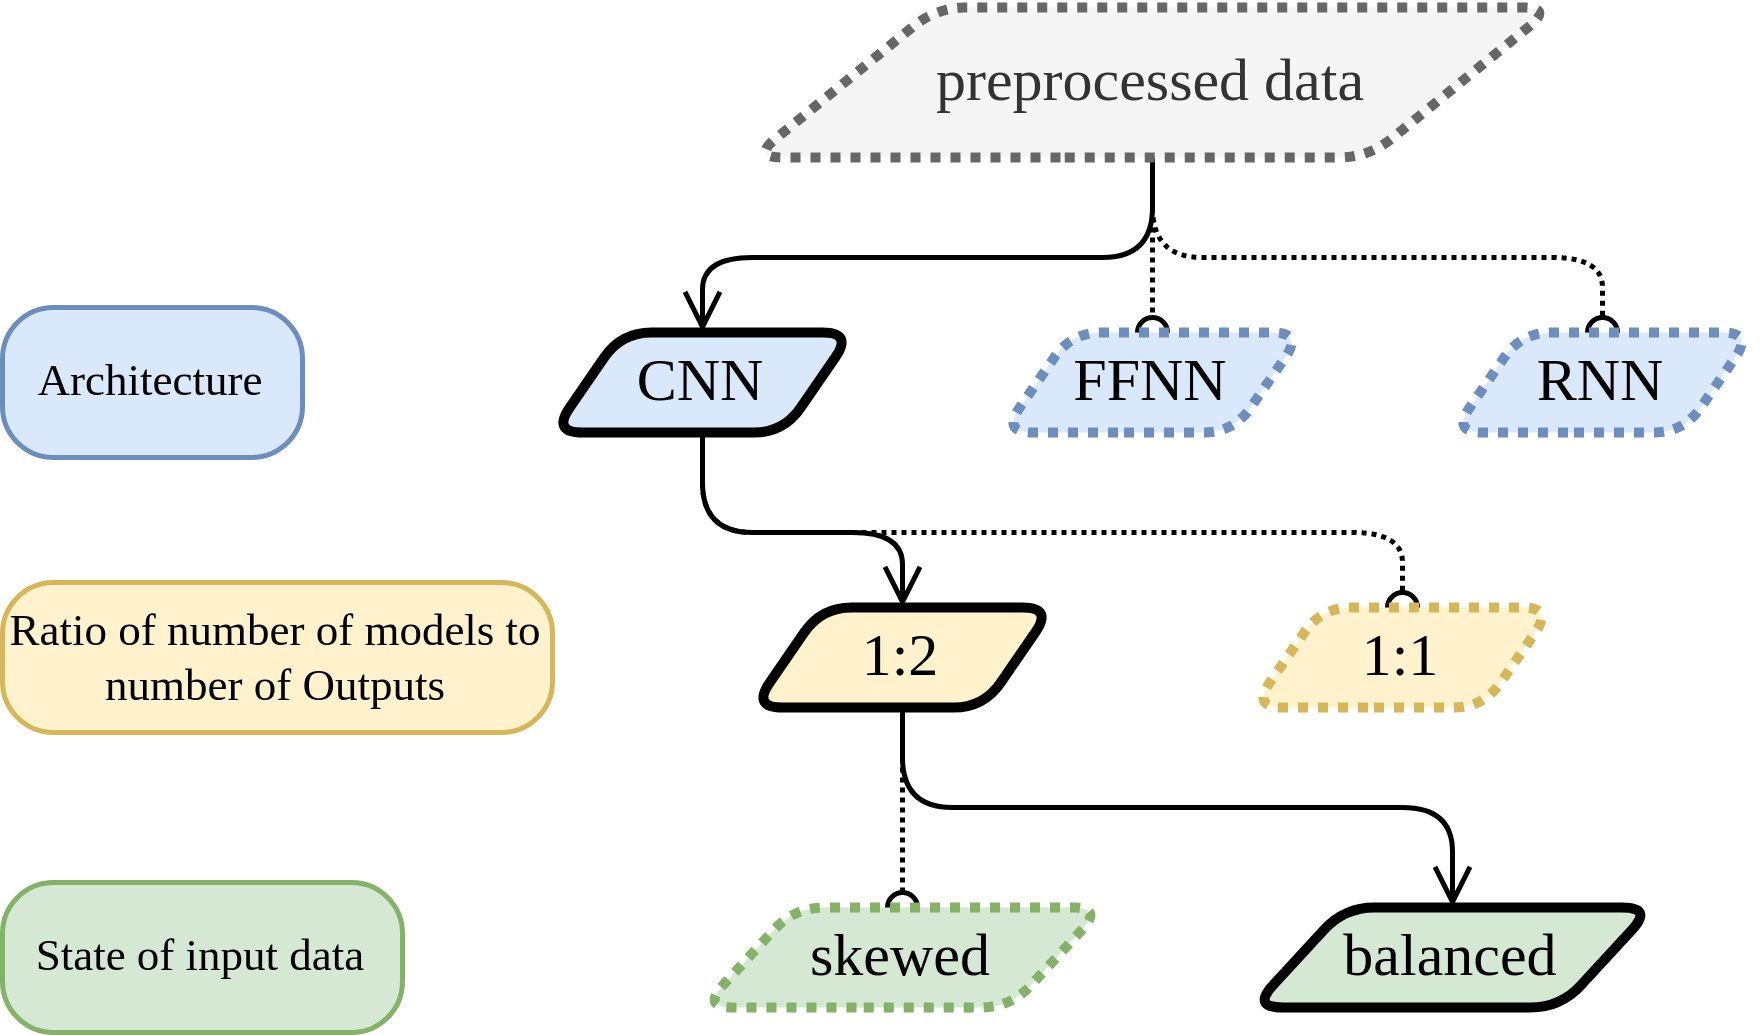
\includegraphics[scale=1.2]{Images/Flowchart.png}
\caption{The work-flow of the project}
\label{flowchart}
\end{center}
\end{figure}
\par

\subsection{Data preprocessing} The data received from the sensors needed to be preprocessed to filter noise and extract relevant data corresponding to the impact. The sensor data from experiments was trimmed between 50 points before and 300 points after the highest peak. The highest peak was considered as this is the point at which the impact vibration reaches the sensor. The isolated data was then normalised and further reduced to zero after the highest peak point. The data was finally filtered using a \emph{\textbf{Savitzky-Golay}} filter to eliminate noise from the processed data. These preprocessed data was then restructured to suit the input of each neural network.     

\subsection{Comparison of the Architecture}
\par
\textbf{Convolutional Neural Network (CNN)}: The CNN consists of 3 convolution layers with 16, 32 and 64 filters respectively. The first layer was activated using a ReLU function, whereas the next two layer were activated using linear function. 1D convolution layers were used for the project, as each sensor produces a one dimensional time series data, and each sensor data is treated as a channel for the given impact data. The final convolved data was passed to a dense hidden layer with 128 neurons which was then output into 2 neurons one each for X and Y coordinate of the received data. A dropout layer and a callback function were introduced into the model in order to avoid an overfit regression model.\\
\textbf{Feed Forward Neural Network (FFNN)}: The FFNN used for this study contains 4 layers with 2 hidden layers, the first hidden layer has 1000 neurons and the following hidden layer contains 326 neurons which was then output into 2 neurons each for predicting the X and Y coordinates for the provided input data. The hidden layers were activated using a \emph{\textbf{Rectified Linear Unit (ReLU)}} function. Callback function was used to monitor the mean squared error (\textbf{MSE}) of the model with a patience of 5 in order to prevent overfitting of the model (similar callback function was used for CNN as well).\\
\textbf{Recurrent Neural Network (RNN)}: The RNN requires some additional preprocessing in order to input the time series in the optimal format. 1 recurrent layer with the LSTM cell type was used which has a state size of 256 and the weights initializer set to \emph{\textbf{HeUniform}}. The layers are bidirectional so that the time series can be read both, forwards and backwards. This was followed by 3 dense layers with the \emph{\textbf{tanh}} activation function whereas a \emph{\textbf{sigmoid}} activation function has been used for the recurrent layer. Callback functions similar to FFNN have been used.

\par
\subsection{Singular model compared to individual models}
\par
CNN provided the best results with minimal variation. This can be attributed to the pattern and feature recognition capability of the CNNs. The CNN architecture was further extended to predict X and Y coordinates of impact location independently using individual NN models, the more accurate of which was further optimised with data balancing. Both the models to independently predict X and Y coordinates had 2,3 and 4 one dimensional filters in the 3 convolution layers used in them, which was then connected to a dense layer with 16 neurons, that further connects to a single output neuron to predict the corresponding impact location coordinate. The model for X uses a kernel window of size \emph{\textbf{(9,1)}} in the first convolution layer, as opposed to the model for Y using a kernel window of \emph{\textbf{(8,1)}} at the same position. On the other hand, prediction using single NN model had a similar structure as used initially while comparing with the FFNN and RNN models.

\par
\subsection{Robustness check}
\par
The selected model was further optimised by balancing data in each quadrant to be used for the training of the neural network. A total of 1024 data files (256 data files corresponding to each quadrant) were available for the training of the NN. Balancing the data helped in reducing the bias of the model towards a specific quadrant such that, it had a fairly constant mean absolute error over all the four quadrants under study.



\section{Results}

Mean absolute error (MAE) was selected as a comparison criteria for different neural network architectures being studied. In CNN, the model was able to predict the impact location with a fairly low MAE, as compared to other architectures. RNN on the other hand had a complex structure, resulting in longer training times. Even then the MAE for RNN was more than double of the other two models used in this study. CNN and FFNN had similar MAE values and so to further compare these two models the mean squared error (MSE) and root mean squared error (RMSE) were also calculated. The RMSE value indicates the variation of the model. Based on the results of FFNN and CNN it was observed that the former had a higher variance as compared to the latter. The error metrics for all the three models are tabulated below (Table~\ref{archCompTab}).

\begin{table}[h!]
\centering
\begin{tabular}{|m{2.3 in}|m{0.95 in}|m{0.95 in}|m{1 in}|}
\hline
\textbf{NN Model} & \textbf{MSE} \textit{($mm^2$)} & \textbf{MAE} \textit{(mm)} & \textbf{RMSE} \textit{(mm)} \\
\hline
\textit{Feed Forward Neural Network} & $470.5735$ & $15.5867$ & $21.6927$\\
\hline
\textit{Convolutional Neural Network} & $234.6247$ & $10.3214$ & $15.3174$\\
\hline
\textit{Recurrent Neural Network} & $1079.8892$ & $25.7841$ & $32.8616$ \\
\hline
\end{tabular}
\caption{Neural Network Architecture Comparison}
\label{archCompTab}
\end{table}
\pagebreak


\noindent
Further extensions of CNN with single and independent models were tested for individual coodrinate's prediction accuracy. The variation in the prediction of the impact location as compared to the desired location with both the CNN models can be seen in the graph plotted below (Fig.~\ref{Actual v/s Predictions Graph}), which plots the desired and predicted coordinates for X and Y independently. Both the graphs are closely overlapping for single CNN model as compared to independent CNN models, indicating a high accuracy of impact location prediction using the selected CNN model (built on single CNN to predict both the X and Y coordinates).

\footnotetext[1]{Quadrant1, Quadrant3 and Quadrant4 Data omitted}
\footnotetext[2]{Quadrant1 and Quadrant3 Data omitted}

\begin{figure}[h!]
\centering
\begin{subfigure}{0.4\textwidth}
%	\centering
	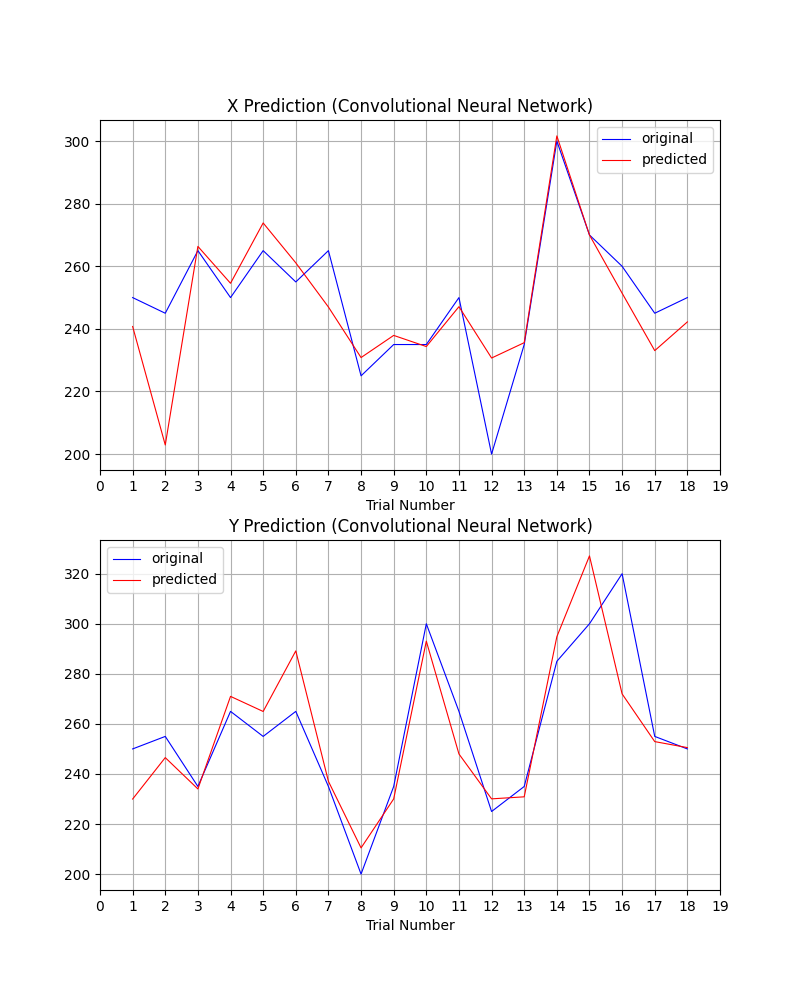
\includegraphics[scale=0.35]{Images/Single CNN prediction.png}
	\caption{Single NN model Predictions}
	\label{One NN model with two outputs}
\end{subfigure}%
\begin{subfigure}{0.4\textwidth}
%	\centering
	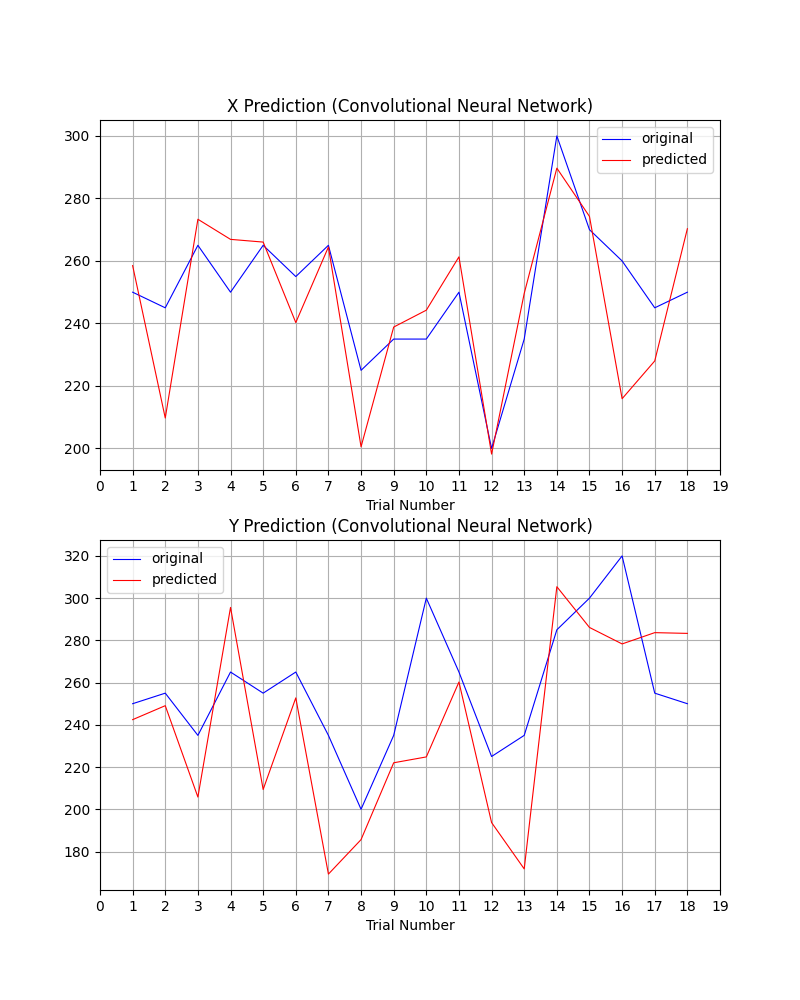
\includegraphics[scale=0.35]{Images/Double CNN prediction.png}
	\caption{Independent NN model Predictions}
	\label{Two NN model each with one output}
\end{subfigure}
\caption{Actual v/s Predicted Impact Co-ordinates Using CNN}
\label{Actual v/s Predictions Graph}
\end{figure}
\vspace{5ex}

\noindent The robustness check was carried out on the better performing CNN (with single NN architecture). Using balanced data as well as data with 0.75\footnotemark[1] and 0.5\footnotemark[2] skewness for training, the robustness of the models was tested. The results of the robustness check are tabulated with the corresponding \textbf{MSE} and \textbf{MAE} values in the table below (Table~\ref{dataBalancing}).




\begin{table}[h!]
\centering
\begin{tabular}{|m{0.95 in}|m{1.5 in}|m{1.5 in}|m{1.5 in}|}
\hline
\textbf{Degree of Skewness} & \textbf{$0\%$\textit{(Balanced Data)}} & \textbf{$75\%$\textit{(Trained on $Q2$ Data)}} & \textbf{$50\%$\textit{(Trained on $Q2$ and $Q4$ Data)}}\\
\hline
\textbf{MSE} \textit{($mm^2$)} & $234.62$ & $500.96$ &$396.34$\\
\hline
\textbf{MAE} \textit{(mm)} & $10.32$ & $18.53$ &$15.06$\\
\hline
\end{tabular}
\caption{Model comparison for completely balanced and skewed data}
\label{dataBalancing}
\end{table}

\section{Discussion}
The results of this study reveal that CNN can be used to predict impact location by measuring the impact vibrations using piezoelectric transducers. CNNs are the best suited NNs to use with such vibrational data, as it is capable of recognizing patterns from the data received from the sensor. CNNs are also able to neglect noise in the data passed to it making it more suitable for use in operation, as it would require minimal data pre-processing. Additionally, the use of this impact vibration data can also be extended to calculate the intensity of impact, which when coupled with the impact location co-ordinate can be further used to calculate stresses generated and stored in the structure over the period of its operation. This would help to continuously monitor the structural health of the system. Thus, enabling us to take preventive measures as soon as an alarm is triggered as a result of detection of deterioration in the structural health/integrity of the system.   

\section{Conclusion}
The study carried out here shows the best fit deep learning model for the prediction of impact position from the sensor data corresponding to it. A CNN using single NN model to predict both the X and Y co-ordinate simultaneously is the best fit ANN for such use case scenario. This is further optimised by training the NN model on balanced data in order to reduce the bias of the model towards any given quadrant. The robustness of the model is checked by training it with data containing no data from any one of the quadrant. From the robustness check it is observed that even when the network is trained with data from only one quadrant, it is still able to predict the impact position with an RMSE of $19.585 mm$ indicating a low variance.   

% References
\begin{thebibliography}{9}
\bibitem{1}
Gaurav Duggal, Venu Gopal Annamdas and Saurab Verma, \emph{"Application of Neural Networks for PiezoelectricSensor
based Strength Monitoring of Concrete Cube"} in Proc. of Int. Conf. on Advances in Design and Construction of Structures,
2012, doi : 02.ADCS.2012.1.518

\bibitem{2}
Lopes V, Park G, Cudney HH, Inman DJ. \emph{Impedance-Based Structural Health Monitoring with Artificial Neural Networks.} Journal of Intelligent Material Systems and Structures. 2000;11(3):206-214. doi:10.1106/H0EV-7PWM-QYHW-E7VF

\bibitem{3}
Iuliana Tabian 1, Hailing Fu 2, and Zahra Sharif Khodaei , \emph{"A Convolutional Neural Network for Impact Detection and
Characterization of Complex Composite Structures"}, Sensors, 19, 4933, Nov.12, 2019, doi : 10.3390/s19224933

\bibitem{4}
Asteris, P.G.; Roussis, P.C.; Douvika, M.G. \emph{Feed-Forward Neural Network Prediction of the Mechanical Properties of Sandcrete Materials.} Sensors 2017, 17, 1344. https://doi.org/10.3390/s17061344

\bibitem{5}
1. Nguyen VQ, Anh TN, Yang H-J. \emph{Real-time event detection using recurrent neural network in social sensors.} International Journal of Distributed Sensor Networks. June 2019. doi:10.1177/1550147719856492

\bibitem{6}
Tan, T.-H.; Lin, Y.-T.; Chang, Y.-L.; Alkhaleefah, M. \emph{Sound Source Localization Using a Convolutional Neural Network and Regression Model.} Sensors 2021, 21, 8031. https://doi.org/10.3390/s21238031
 
\end{thebibliography}
 
\end{document}


